\documentclass[aspectratio=169,11pt]{beamer}
\usetheme{default}
\usecolortheme{seahorse}
\setbeamertemplate{navigation symbols}{}
\setbeamertemplate{footline}[frame number]
\usepackage{booktabs,amsmath,amssymb}
\graphicspath{{figures/}}
\newcommand{\E}{\mathbb{E}}
\definecolor{good}{HTML}{1B7F3B}
\definecolor{bad}{HTML}{B22222}

\title{Reward Shaping Is Noise Shaping}
\subtitle{and a law for the accuracy--diversity frontier of RLVR}
\author{Mohamed Ayman}
\date{October 23, 2026 --- status}

\begin{document}
\frame{\titlepage}

\begin{frame}{The question}
\begin{itemize}
\item RL with verifiable rewards: sample answers, a checker grades them, update $g=\sum_i A_i\nabla\log\pi(y_i)$.
\item Many papers change the advantage $A_i$ (reward right only, penalize wrong only, baselines, pass@$k$ weights, entropy bonuses) and report more \textbf{diversity} (pass@$k$).
\item They compare methods \textbf{at the same training step}. A slower method is less sharpened there, so it \emph{looks} more diverse.
\item Our question: is the diversity real? The fair test is \textbf{pass@$k$ at matched pass@1}.
\end{itemize}
\end{frame}

\begin{frame}{Theory: same direction, different noise}
For any rule that scores answers only by correctness ($p$: a question's success rate)
\[\E g=c(p)\,\nabla p,\qquad \E\|g\|^2=F_1D_1(p)+F_0D_0(p)+\|\nabla p\|^2X(p)\]
\begin{itemize}
\item A rule can only reweight questions and change the noise; wrong answers carry most of it (2--3$\times$).
\item Noise sets the \textbf{speed} along one accuracy--diversity curve, not the curve.
\item At matched pass@1, pass@$k=\E_x[1-(1-p_x)^k]$: diversity is how evenly success is spread across questions.
\end{itemize}
\end{frame}

\begin{frame}{Diagnosis 1: one curve, two model families}
\centering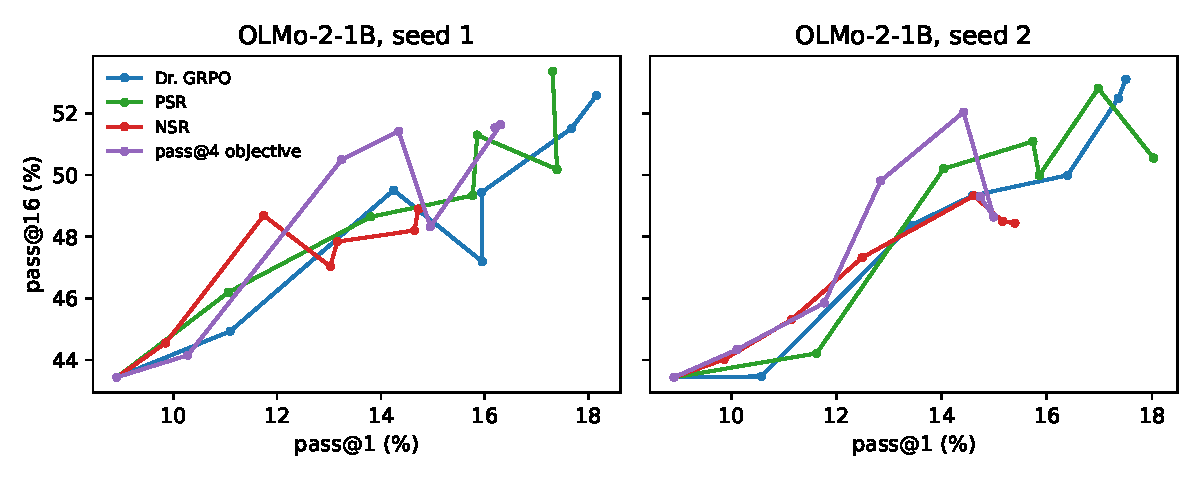
\includegraphics[width=0.85\linewidth]{olmo_curves.pdf}\\[4pt]
\small OLMo-2-1B: NSR minus PSR at matched accuracy $-0.30$, 90\% $[-1.28,+0.77]$: equivalent within $\pm2$. Same on Qwen for PSR, NSR, five baselines, the NSR paper's code, a pass@4 objective.
\end{frame}

\begin{frame}{Diagnosis 2: the noise is the cause}
\begin{columns}
\column{0.55\linewidth}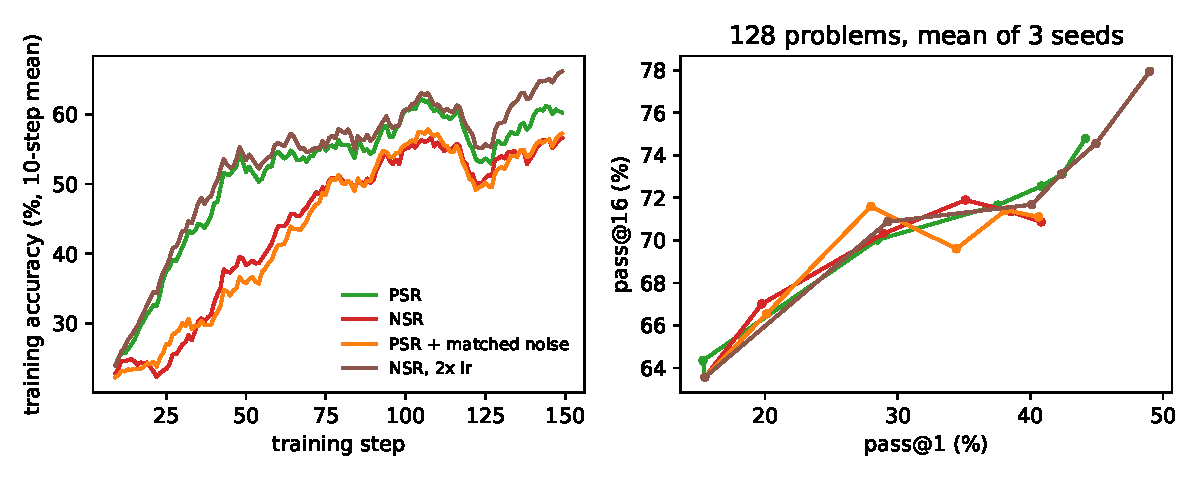
\includegraphics[width=\linewidth]{noise_test.pdf}
\column{0.45\linewidth}\small
\begin{itemize}
\item Add zero-mean noise of NSR's size to PSR.
\item \textbf{PSR + noise is as slow as NSR}: $\phi=-0.11$ $[-0.22,-0.05]$ (NSR $=0$, PSR $=1$).
\item NSR at 2$\times$ learning rate recovers.
\item Not temperature either: a late checkpoint sampled hotter does not beat the curve ($-1.42$).
\end{itemize}
\end{columns}
\end{frame}

\begin{frame}{Trying to move the curve}
\small\centering
\resizebox{\linewidth}{!}{\begin{tabular}{@{}lll@{}}
\toprule
Method & pass@16 at matched accuracy & \\
\midrule
Reward shaping, entropy, unlikeliness, pass@$k$ objective & $\approx0$ & finished\\
Replay of own successes (coverage-weighted) & $+1.19$ $[+0.54,+1.79]$ & finished\\
Replay seeded with base-model successes & $+1.02$; 5.4 points less accurate & finished\\
Annealed replay; MaxRL + group completion (pilot) & $+1.3$; $+1.1$; 6.5 less accurate & interim\\
Group completion; prefix-guided rollouts (pilot) & -- & evaluating\\
\textbf{Warm start} (fine-tune on base successes, then RL) & \textbf{beyond Dr.\ GRPO's range} & \\
\textbf{Groups of 32} (4$\times$ samples) & \textbf{beyond Dr.\ GRPO's range} & 2 of 3 seeds\\
\bottomrule
\end{tabular}}\\[6pt]
Inside RL, everything sits near $+1$, below our $+2$ bar.
\end{frame}

\begin{frame}{Where the gains go}
\begin{columns}
\column{0.48\linewidth}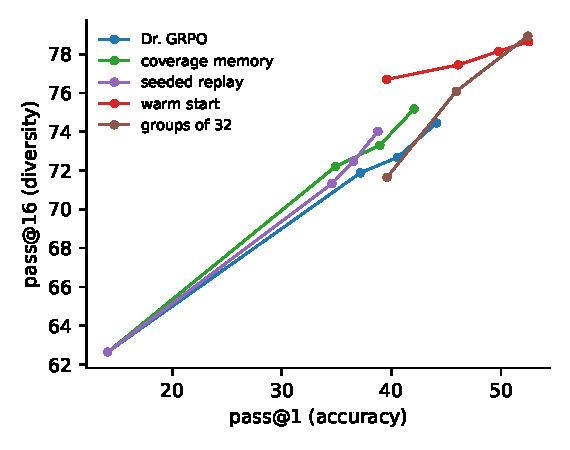
\includegraphics[width=\linewidth]{frontier_qwen.pdf}
\column{0.52\linewidth}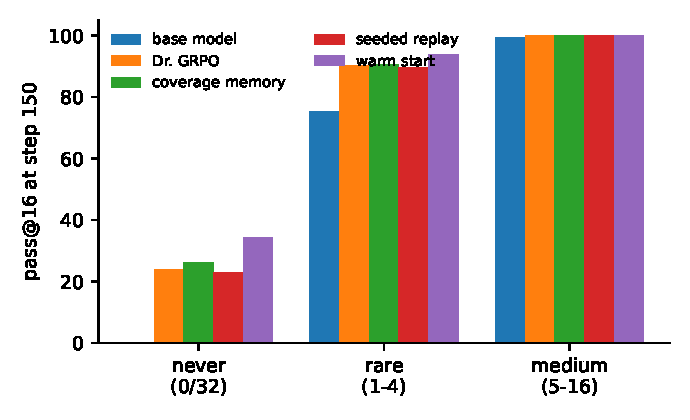
\includegraphics[width=\linewidth]{strata.pdf}
\end{columns}
\small Warm start and groups of 32 end at the same point (pass@1 52.5, against 44.1 for Dr.\ GRPO). The warm start's pass@16 gain sits on problems the base never solves (24 $\to$ 34). At 1,024 tokens all numbers rise (Dr.\ GRPO pass@1 57.7 vs 44.6): the 512-token budget matters.
\end{frame}

\begin{frame}{New: a law for the frontier}
\begin{block}{Per-question log-odds learning from base counts}
\[\theta_x(0)=\log\tfrac{c_x+a}{n-c_x+b},\qquad \dot\theta_x=p_x(1-p_x)+\tau\,\overline{p(1-p)}\]
\end{block}
\begin{itemize}
\item Inputs: the base model's per-question success counts; each checkpoint's pass@1 (sets progress $t$).
\item $\tau=-0.20$ fitted once on Dr.\ GRPO, then \textbf{frozen} (pre-registered).
\item Predicts the whole distribution: pass@$k$ for all $k$, difficulty strata, per-question counts.
\item Diversity collapse = \textbf{rich get richer}: a uniform improvement would put never-solved problems at 70--80 pass@16; observed 24.
\end{itemize}
\end{frame}

\begin{frame}{The law, tested prospectively}
\begin{columns}
\column{0.42\linewidth}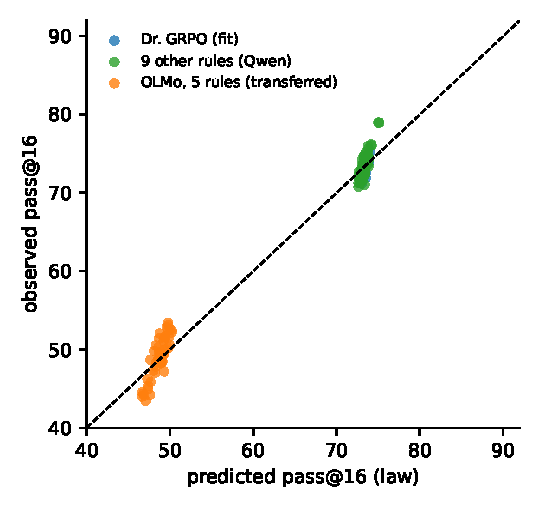
\includegraphics[width=\linewidth]{law_fit.pdf}
\column{0.58\linewidth}\small
\resizebox{\linewidth}{!}{\begin{tabular}{@{}lcc@{}}
\toprule
Test set & RMSE pass@16 & verdict\\
\midrule
9 other rules, Qwen (56) & \textbf{1.21} & \textcolor{good}{supported}\\
OLMo, $\tau$ from Qwen (50) & \textbf{1.90} & \textcolor{good}{supported}\\
1,024 tokens (4) & \textbf{0.85} & \textcolor{good}{supported}\\
Warm start (9) & 3.56 & \textcolor{bad}{falsified}\\
450 steps & running & \\
\bottomrule
\end{tabular}}\\[4pt]
Alternatives: uniform shift 10--21, affine 1.3--12.6; the law wins in per-question likelihood in 117/119 checkpoints.
\end{columns}
\end{frame}

\begin{frame}{What the law says}
\begin{itemize}
\item From a base model, the frontier is set by \textbf{base difficulty} and near-independent per-question learning; reward rules only change how far along it a run gets.
\item That is why reward shaping cannot move it. Only two levers can: the \textbf{starting distribution} (information on rare questions) and \textbf{transfer} between questions.
\item \textbf{The warm start breaks the law}: afterwards RL lifts never-solved problems 12 points less than predicted (fitted $\tau\approx-0.7$): fine-tuning changes the dynamics.
\item Against the law's extended frontier the warm start sits $+3.4$ above and groups of 32 reaches $+3.9$; the 450-step run decides whether that is real.
\end{itemize}
\end{frame}

\begin{frame}{Position in the 2026 literature}
\small
\begin{columns}[T]
\column{0.5\linewidth}
\textbf{Ours, unpublished}
\begin{itemize}
\item noise sets speed along one curve
\item NSR on PSR's curve, two families
\item the noise-injection causal test
\item matched-accuracy protocol
\item temperature does not beat the curve
\item a prospective frontier law
\end{itemize}
\column{0.5\linewidth}
\textbf{Published, to cite or answer}
\begin{itemize}
\item same direction, per-question weight (Davis \& Recht; Heckel et al.)
\item base-seeded replay (TAR); coverage weight (BBG)
\item rescue of all-wrong groups (LSPO, LUFFY)
\item transfer curricula (TAC, GradAlign)
\item ``RLVR is a Kernel'': strongest challenge to the law
\end{itemize}
\end{columns}
\vspace{4pt}
No 2026 method paper compares at matched accuracy.
\end{frame}

\begin{frame}{Where we stand}
\small
\resizebox{\linewidth}{!}{\begin{tabular}{@{}lll@{}}
\toprule
Stage & Independent review & Why\\
\midrule
Diagnosis only & 5/10 & solid, but the theory is partly prior work\\
+ law passes prospective tests & \textbf{7/10} & a new, predictive result\\
+ method that improves the frontier across scales & 8/10 & diagnosis $\to$ law $\to$ method\\
\bottomrule
\end{tabular}}
\vspace{6pt}
\begin{itemize}
\item \textbf{Running:} 450-step Dr.\ GRPO (law beyond its fit); deep base sampling (sign of $\tau$); TAR, BBG, MaxRL, W-REINFORCE at matched accuracy; pilot evaluations; 1,024-token and transfer checks.
\item \textbf{Method candidate from the law:} spend demonstration acquisition where the law predicts stalls, against random allocation and the warm start at equal compute.
\end{itemize}
\end{frame}

\end{document}
